\documentclass{anschreiben}

\usepackage{wrapfig}

\renewcommand{\deinName}{Ingo Blechschmidt und Rolf Wittmann}
\renewcommand{\deineMailAdresse}{iblech@speicherleck.de und rkw95@web.de}


\renewcommand{\datum}{\today}
\renewcommand{\betreff}{Matheschülerzirkel der Universität Augsburg}

\begin{document}

\newcommand{\direuch}{}

\newread\quelle
\openin\quelle=teilnehmende.csv
\read\quelle to \zeile

\loop
\read\quelle to \zeile
\ifeof\quelle\global\morefalse\else

\bearbeitezeile

\ifganzeklasse Liebe Schülerinnen und Schüler,\else
\ifweiblich Liebe\else Lieber\fi{} \vorname,\fi

\renewcommand{\direuch}{\ifganzeklasse euch\else dir\fi}

habt ihr schon von Paul Erdős gehört? Das war einer der bedeutendsten
Mathematiker des letzten Jahrhunderts. Er zog von Mathematiker zu Mathematiker
und löste mit ihnen gemeinsam zahlreiche schwere Probleme. Über ihn wird
folgendes berichtet:

\begin{quote}
Was wäre, wenn technologisch weit fortgeschrittene Aliens bei uns landen
und uns auffordern würden, ihnen den Wert der Zahl~$R(5,5)$ mitzuteilen, wenn
sie nicht die Erde zerstören sollen? Für diesen Fall meinte Erdős, dass wir all
unsere Computer und Mathematiker an das Problem setzen sollten. Wenn sie aber
nach~$R(6,6)$ verlangen würden, sollten wir lieber einen hoffnungslosen
Präventivschlag ausüben -- so schwierig ist es,~$R(6,6)$ zu berechnen.
\end{quote}

Was ist diese Zahl~$R(6,6)$, die uns Erdős zu Folge ewig verschlossen bleiben
wird? Möglicherweise denkt ihr an eine absurd große Zahl. Tatsächlich aber weiß
man schon, dass sie zwischen 102 und 165 liegt (jeweils eingeschlossen). Sie
hat unter all diesen Zahlen eine ganz besondere Eigenschaft.

Im beiliegenden Zirkelbrief geht es um Zahlen dieser Art und allgemeiner um
große und schwer zu berechnende Zahlen. Wir hoffen, dass euch der Brief
gefällt, und bitten euch, all eure Kommentare und Fragen an uns zu schicken.

Es tut uns leid, dass ihr so lange auf diesen Brief warten musstet. Ab jetzt
wird der Rhythmus wieder regelmäßiger sein.

Viele Grüße

Ingo und Rolf
\enlargethispage{2em}

\vspace*{-2em}

\begin{center}
  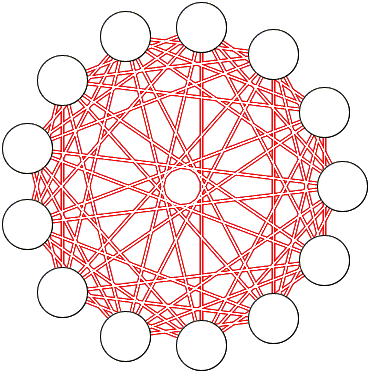
\includegraphics[width=0.3\textwidth]{ramsey}

  \tiny $R(5,3) = 14$. Von https://tinyurl.com/y77p9qoy
\end{center}

PS: Am 26. Mai findet bei uns auf dem Campus der \emph{Mai-Mathetag} statt.
Schaut vorbei, wenn er euch interessiert!

\newpage
\fi\ifmore\repeat

\closein\quelle

\end{document}
